

\chapter{Introduction}

% \section{Motivation}
% In the span of the past three decades, the internet has blossomed into an indispensable facet of our daily existence. From the ubiquitous presence of smartphones, which have become synonymous with connectivity, to the unexpected convergence with unconventional devices such as internet-connected cow milking apparatus, the internet has woven itself intricately into the fabric of modern life. This project embarks upon a daring experiment, seeking to address a profound question: can a student from the year 2023 harness the ingenuity possessed by the geniuses of the past half-century, and engineer a fully functional communication network, all the while leveraging on the readily available hardware and the wealth of knowledge graciously bestowed upon him by these very pioneers?

\section{Structural Overview}

\begin{figure}[H]
\begin{center}
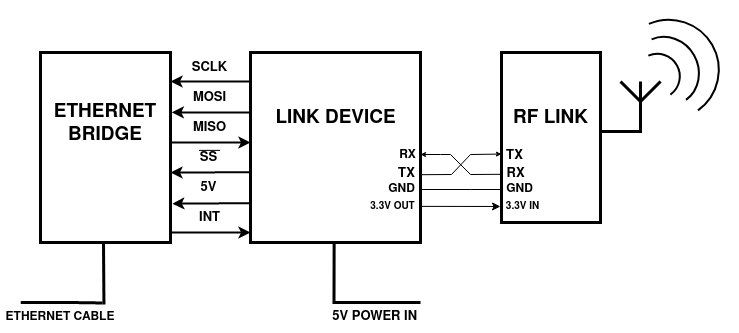
\includegraphics[width=1\textwidth]{schematic-diagram}
\end{center}
\caption{Schematic Diagram of a Single Agent.}
\label{fig-pin}
\end{figure}

In the current form, the system is designed so as to facilitate communication between two agents. Both have three main hardware components: Link device, Ethernet bridge, and RF link. The main computational unit, which handles most of the data processing, is the Link device. The Ethernet bridge is used to provide Ethernet connectivity to the Link device, as it misses the necessary hardware interface. The Ethernet bridge is running stock firmware with no addition software written for it. 
The connection between Link device and Ethernet bridge is facilitated via SPI. The last component is the RF link, the sole purpose of which, is to perform the data transmission over RF. The communication between Link device and the RF link is maintained via UART. The functionality of RF link is abstracted away, so the Link devices are operating as if they are directly connected to each other. Even though there is only one Ethernet interface on both agents, both sides can provide connectivity to multiple network user devices if they are connected through a network switch or hub. Currently, we have an arbitrary limitation of 16 clients on each side, but even fewer number of clients would not be able to use the network, because of the modest network throughput.

% \newpage

As the purpose of our system is Network Bridging, data from one end interface to another passes over 6 components:
\begin{enumerate}[nolistsep]
    \item Transmitter side's Ethernet bridge,
    \item Transmitter side's Link device,
    \item Transmitter side's RF link,
    \item Receiver side's RF link,
    \item Receiver side's Link device,
    \item Receiver side's Ethernet bridge.
\end{enumerate}

This causes a demand for packet nesting structure. Figure \ref{packet-nesting} illustrates that structure.

\begin{figure}[H]
\begin{center}
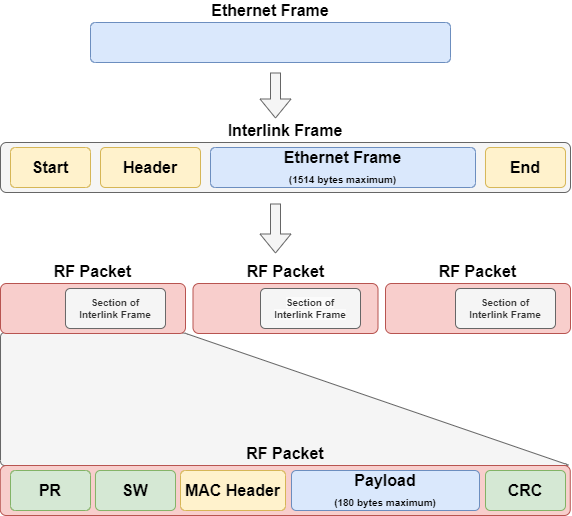
\includegraphics[width=0.8\textwidth]{packet-nesting.png}
\end{center}
\caption{Overview of System's Packet Nesting Structure.}
\label{packet-nesting}
\end{figure}

The whole source code of the project is available on \href{https://github.com/Tigran-teq-Tadevosyan/TIR}{Github} \footnote{https://github.com/Tigran-teq-Tadevosyan/TIR}.


\section{Hardware}
\begin{enumerate}[nolistsep]
\item PIC32MZ DA Curiosity Development Kit (Link device),
\item TI Lunchpad kit with CC1312R1 MCU	(RF link),			
\item JESSINIE board with W5500 embedded Ethernet controller (Ethernet bridge),
\item Rigol DS1102E Digital Oscilloscopes \footnote[1]{For debugging purposes and for some of the screenshots included in this report.}.
\end{enumerate}

\section{Software}
\begin{enumerate}[nolistsep]
\item MPLAB X IDE v6.05,
\item MPLAB IPE v6.05,
\item MPLAB XC32 Compiler v4.21,
\item Code Composer Studio v12.3.0,
\item GCC v9.2.1 (Linaro) \footnote[2]{Version for AMD64 to ARM cross-compilation.},
\item TI Lunchpad kit with CC1312R1 MCU,
\item Wireshark v12.3.0 \footnote[3]{For debugging purposes and for some of the screenshots included in this report.}.
\end{enumerate}